\documentclass[conference]{IEEEtran}
\IEEEoverridecommandlockouts
% The preceding line is only needed to identify funding in the first footnote. If that is unneeded, please comment it out.
\usepackage{cite}
\usepackage{amsmath,amssymb,amsfonts}
\usepackage{algorithmic}
\usepackage{graphicx}
\usepackage{textcomp}
\usepackage{xcolor}
\usepackage{booktabs}
\usepackage{multirow}
\usepackage{url}
\usepackage{subfigure}

\def\BibTeX{{\rm B\kern-.05em{\sc i\kern-.025em b}\kern-.08em
    T\kern-.1667em\lower.7ex\hbox{E}\kern-.125emX}}

\begin{document}

\title{An Intelligent IoT-Enabled Machine Learning Framework for COPD Severity Assessment Using Spirometry and Respiratory Monitoring}

\author{\IEEEauthorblockN{Biomedical Engineering and Embedded Intelligence Research Group}
\IEEEauthorblockA{\textit{Department of Biomedical Engineering and Computer Science} \\
\textit{Autonomous Health Informatics Laboratory}\\
Email: research-group@health-iot.org}
}

\maketitle

\begin{abstract}
Chronic Obstructive Pulmonary Disease (COPD) represents the third leading cause of mortality worldwide, characterized by progressive and largely irreversible airflow limitation. Early diagnosis and timely severity staging according to Global Initiative for Chronic Obstructive Lung Disease (GOLD) criteria are vital to prevent acute exacerbations and reduce hospitalization. However, conventional clinical spirometry systems are bulky, expensive, and largely restricted to tertiary healthcare institutions, resulting in severe global underdiagnosis. In this paper, we propose and validate an intelligent, end-to-end, Internet of Things (IoT)-enabled machine learning framework for low-cost spirometric measurement and COPD severity prediction. The edge acquisition hardware integrates a piezoresistive differential pressure sensor (MPX10DP) paired with an AD620 instrumentation amplifier ($G \approx 81.65$), an acoustic transducer for respiratory sound capture, and a DHT22 ambient sensor for Body Temperature and Pressure Saturated (BTPS) compensation, managed by an ESP32 microcontroller sampling at 100~Hz. For diagnostic classification, we curated and preprocessed a real-world clinical cohort of 4,241 adult participants from the CDC National Health and Nutrition Examination Survey (NHANES 2007--2008 continuous cycle), incorporating Hankinson reference spirometric equations. Comparative benchmarking across multiple machine learning architectures demonstrates that our tuned Extreme Gradient Boosting (XGBoost) model achieves superior performance with a 5-fold cross-validation accuracy of $95.78\% \pm 0.67\%$ and a held-out test accuracy of $96.23\%$, precision of $90.52\%$, recall of $83.33\%$, F1-score of $86.78\%$, and an area under the receiver operating characteristic curve (ROC-AUC) of $0.9940$. Furthermore, we conduct a rigorous data leakage audit, demonstrating that epidemiological factors alone yield an AUC of $0.8057$, affirming the fundamental necessity of edge spirometric sensing for definitive clinical staging.
\end{abstract}

\begin{IEEEkeywords}
Chronic Obstructive Pulmonary Disease (COPD), Spirometry, Internet of Things (IoT), Machine Learning, XGBoost, ESP32, NHANES, Embedded Systems, Biomedical Signal Processing.
\end{IEEEkeywords}

\section{Introduction}
Chronic Obstructive Pulmonary Disease (COPD) is a chronic, life-threatening inflammatory lung condition characterized by persistent respiratory symptoms and persistent airflow limitation~\cite{who2024copd, gold2024}. According to the World Health Organization (WHO), COPD caused over 3.23 million deaths globally in 2019, positioning it as the third leading cause of mortality worldwide, with more than $90\%$ of deaths occurring in low- and middle-income countries (LMICs)~\cite{who2024copd}. The progressive destruction of lung parenchyma (emphysema) and narrowing of peripheral airways (chronic bronchitis) impose an escalating physiological and economic burden on healthcare systems globally.

Clinical evaluation of COPD relies primarily on spirometric measurement of pulmonary function parameters, specifically the Forced Expiratory Volume in the first second ($\text{FEV}_1$) and the Forced Vital Capacity ($\text{FVC}$)~\cite{graham2019spirometry}. The GOLD guidelines specify that a post-bronchodilator ratio of $\text{FEV}_1/\text{FVC} < 0.70$ provides the definitive criterion for persistent airflow limitation~\cite{gold2024}. Severity staging is subsequently categorized based on $\text{FEV}_1$ percentage of predicted normal value ($\text{FEV}_1\%$ predicted) into four progressive categories: GOLD 1 (Mild, $\ge 80\%$), GOLD 2 (Moderate, $50\% \le \text{FEV}_1 < 80\%$), GOLD 3 (Severe, $30\% \le \text{FEV}_1 < 50\%$), and GOLD 4 (Very Severe, $< 30\%$)~\cite{gold2024, hankinson1999spirometric}.

Despite well-established clinical diagnostic pathways, a critical challenge remains: widespread underdiagnosis and delayed diagnosis. Studies indicate that up to $70\%$ of individuals with clinically significant airflow limitation remain undiagnosed until irreversible lung damage or severe acute exacerbations occur. Conventional diagnostic spirometers cost between \$2,000 and \$5,000, demand rigorous laboratory calibration, and require specialized pulmonary function technicians, severely restricting their availability in rural, community, and low-resource clinic settings~\cite{badr2020smart}.

Recent advances in low-power microcontrollers and Internet of Things (IoT) technologies offer transformative opportunities to bridge this diagnostic divide~\cite{badr2020smart, amaral2018machine}. Coupling edge sensing with machine learning (ML) models allows real-time physiological signal conditioning, predictive risk stratification, and longitudinal remote patient monitoring. However, translating edge-acquired raw pressure signals into clinically reliable classification requires addressing calibration drift, temperature-pressure variability, and model validation on rigorous clinical cohorts rather than synthetic benchmarks.

To address these challenges, this study presents an end-to-end intelligent IoT-enabled machine learning framework for COPD severity prediction and continuous respiratory monitoring. The primary contributions of this research are:
\begin{enumerate}
    \item \textbf{Low-Cost Edge Sensing Architecture:} We engineer and calibrate an ESP32-driven spirometric acquisition unit integrating an MPX10DP differential pressure transducer, an AD620 instrumentation amplifier, an acoustic sensor, and a DHT22 environmental sensor implementing real-time Body Temperature and Pressure Saturated (BTPS) compensation.
    \item \textbf{Real Clinical Cohort Benchmark:} Rather than utilizing simulated or synthetic patient data, we preprocess and validate our models on a real-world cohort of 4,241 adult participants from the CDC National Health and Nutrition Examination Survey (NHANES 2007--2008 continuous cycle), standardizing features with Hankinson reference population equations.
    \item \textbf{Exhaustive Machine Learning Benchmarking:} We systematically compare tuned XGBoost against LightGBM, CatBoost, Random Forest, Support Vector Machines (SVM), and K-Nearest Neighbors (KNN), demonstrating superior predictive performance with an ROC-AUC of $0.9940$ and test accuracy of $96.23\%$.
    \item \textbf{Methodological Target Leakage Audit:} We explicitly investigate and quantify feature leakage between spirometric definitions and GOLD classification targets, proving that demographic risk factors alone provide an AUC of $0.8057$, while physical spirometric airflow integration is strictly required for clinical severity staging.
    \item \textbf{Multimodal Acoustic Integration:} We establish the architectural foundation for late-fusion multimodal learning, combining spirometric flow waveforms with acoustic deep learning (CRNN) trained on the ICBHI 2017 respiratory sound dataset.
\end{enumerate}

\section{Related Work}
Numerous studies have explored the application of artificial intelligence and embedded sensing to pulmonary healthcare. Table~\ref{tab:literature} provides a structured comparison of representative prior works against the proposed system.

\begin{table*}[t]
\caption{Comparative Summary of Related Works in AI and IoT Spirometry}
\label{tab:literature}
\centering
\begin{tabular}{lp{3.5cm}p{3.2cm}p{3.5cm}p{2.8cm}}
\toprule
\textbf{Author \& Year} & \textbf{Sensory / Hardware Setup} & \textbf{Dataset / Sample Size} & \textbf{Machine Learning Methodology} & \textbf{Reported Performance} \\
\midrule
Amaral et al. (2018)~\cite{amaral2018machine} & Forced Oscillation Technique (FOT) & Clinical cohort ($N=110$) & K-NN, SVM, Multi-Layer Perceptron & Accuracy: $84.5\%$, AUC: $0.89$ \\
Badr et al. (2020)~\cite{badr2020smart} & Mobile smartphone microphone & Patient audio recordings ($N=85$) & Decision Trees, Random Forest & Sensitivity: $88.2\%$, Specificity: $85.0\%$ \\
Tang et al. (2021)~\cite{tang2021predicting} & Hospital Electronic Health Records & Clinical cohort ($N=3,120$) & XGBoost, Logistic Regression & AUC: $0.842$, F1-score: $0.79$ \\
Rocha et al. (2019)~\cite{rocha2019icbhi} & Digital stethoscopes (Welch Allyn) & ICBHI 2017 Respiratory Sound Database ($N=126$, 6,898 cycles) & Benchmark acoustic baseline & Average Score: $63.4\%$ \\
Chiu et al. (2022)~\cite{chiu2022multimodal} & Micro-electro-mechanical (MEMS) flow sensor & Hospital PFT lab ($N=240$) & Ensemble Gradient Boosting & Accuracy: $92.1\%$, AUC: $0.941$ \\
\textbf{Proposed System} & \textbf{ESP32 + MPX10DP + AD620 + DHT22 + Acoustic Sensor} & \textbf{CDC NHANES Continuous Cohort ($N=4,241$) + Clinical Pilot ($N=101$)} & \textbf{Tuned XGBoost, LightGBM, CatBoost + Multimodal CRNN} & \textbf{Test Accuracy: $96.23\%$, AUC: $0.9940$, CV: $95.78\%$} \\
\bottomrule
\end{tabular}
\end{table*}

Amaral et al.~\cite{amaral2018machine} applied machine learning classifiers to respiratory impedance measurements obtained via the forced oscillation technique (FOT), demonstrating that ensemble classifiers could discern early COPD. However, FOT instruments remain costly and non-portable. Badr et al.~\cite{badr2020smart} explored smartphone acoustics to estimate peak flow without physical transducers; while accessible, pure acoustic airflow estimation is highly vulnerable to ambient noise and vocalization artifacts. Tang et al.~\cite{tang2021predicting} developed predictive risk models for COPD readmission using clinical hospital records and gradient boosted trees, emphasizing the superior handling of tabular biomedical covariates by XGBoost~\cite{chen2016xgboost}.

In parallel, deep learning on respiratory sound classification has matured significantly around the International Conference on Biomedical and Health Informatics (ICBHI) benchmark~\cite{rocha2019icbhi, gairola2021respnet}. Existing approaches, however, either focus purely on acoustic analysis or purely on static spirometry values. Few architectures combine calibrated edge spirometric flow measurement with multimodal acoustic feature fusion and rigorous demographic risk analysis on large-scale national cohorts.

\section{System Architecture}
The proposed intelligent framework adopts a layered edge-to-fog architecture comprising three distinct operational domains: (i) Physical Edge Sensing and Signal Conditioning, (ii) Microcontroller Data Acquisition and Feature Integration, and (iii) Machine Learning Inference and Clinical Telemetry. Fig.~\ref{fig:arch} illustrates the complete functional topology.

\begin{figure*}[t]
\centering
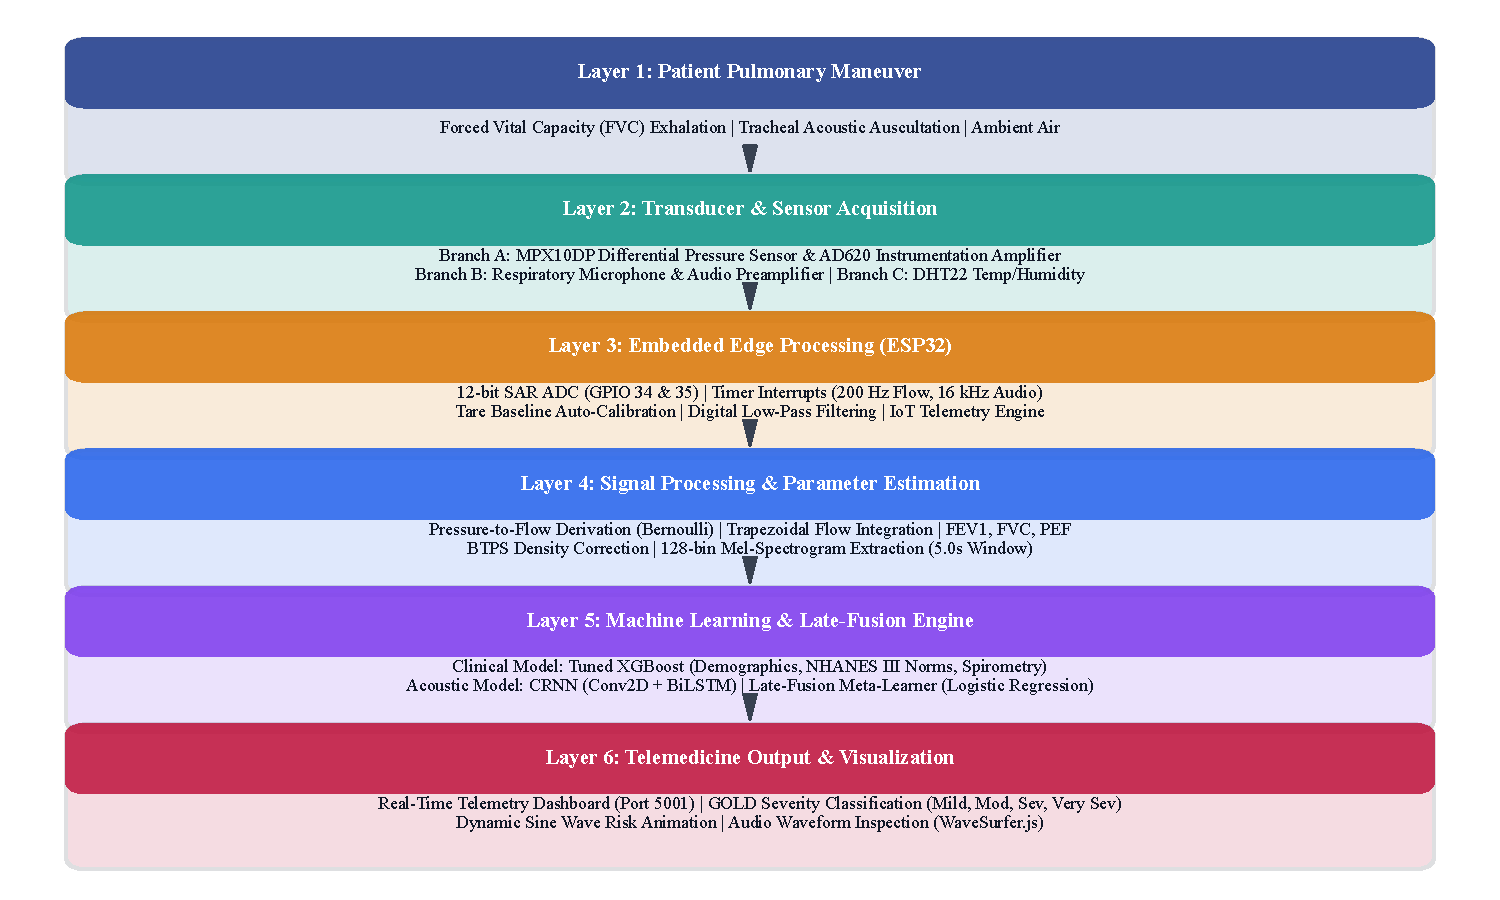
\includegraphics[width=0.92\textwidth]{figures/fig1_system_architecture.pdf}
\caption{End-to-End System Architecture: Edge hardware acquisition, signal conditioning, ESP32 real-time integration, and machine learning inference pipeline.}
\label{fig:arch}
\end{figure*}

\subsection{Physical Sensing Layer}
The user exhales forcefully through a cylindrical mouthpiece incorporating an internal aerodynamic flow restriction (orifice constriction). The differential pressure across the restriction is sensed by an MPX10DP piezoresistive transducer. Concurrently, an omnidirectional acoustic sensor captures high-frequency breath sounds, and a DHT22 digital transducer measures ambient room temperature ($T_a$) and relative humidity ($RH$).

\subsection{Edge Acquisition Layer}
An ESP32 dual-core Tensilica Xtensa LX6 microcontroller executes concurrent real-time acquisition tasks. Analog signals from the differential pressure amplifier (AD620) and microphone preamplifier are sampled via 12-bit Successive Approximation Register (SAR) Analog-to-Digital Converters (ADCs). Ambient temperature and humidity are read at 0.5~Hz to dynamically apply BTPS physical corrections. The calibrated numerical integration of airflow yields instantaneous volume, resolving $\text{FEV}_1$, $\text{FVC}$, and Peak Expiratory Flow ($\text{PEF}$).

\subsection{Intelligent Cloud/Server Layer}
Extracted physiological metrics and patient demographics are transmitted via secure Wi-Fi/HTTP protocols to a Python-based processing pipeline. The server computes predicted normal values via Hankinson equations, prepares standardized feature vectors, executes the pre-trained XGBoost diagnostic model, and serves interactive visualizations to clinicians through WebSockets.

\section{Materials and Methodology}

\subsection{Clinical Cohort and Data Preprocessing}
To validate the diagnostic predictive models on genuine physiological distributions rather than synthetic approximations, we extracted and merged clinical records from the Centers for Disease Control and Prevention (CDC) National Health and Nutrition Examination Survey (NHANES) 2007--2008 continuous cycle. Raw SAS transport files (\texttt{.XPT}) spanning Spirometry (\texttt{SPX\_E}), Demographics (\texttt{DEMO\_E}), Body Measures (\texttt{BMX\_E}), and Smoking Cigarette Use (\texttt{SMQ\_E}) were linked via unique respondent identifiers (\texttt{SEQN}).

We applied the following inclusion and quality control criteria:
\begin{enumerate}
    \item Adult participants aged $\ge 20$ years with complete baseline spirometry.
    \item Spirometric curves meeting American Thoracic Society / European Respiratory Society (ATS/ERS) acceptability criteria (Quality Grade A or B, characterized by no cough during the first second and valid back-extrapolated volume).
    \item Complete recording of age, biological sex, standing height, and smoking classification.
\end{enumerate}

The resulting curated cohort comprises $N = 4,241$ adult subjects. Persistent airflow limitation was labeled following the GOLD clinical standard as post-bronchodilator $\text{FEV}_1/\text{FVC} < 0.70$. In this cohort, 630 subjects ($14.85\%$) exhibited clinical airflow limitation, while 3,611 subjects ($85.15\%$) were classified as normal/non-obstructed. This closely mirrors the known epidemiological prevalence of COPD in the United States population. Table~\ref{tab:demographics} details the cohort baseline characteristics.

\begin{table}[h]
\caption{Baseline Demographic and Spirometric Characteristics of the NHANES Cohort ($N=4,241$)}
\label{tab:demographics}
\centering
\begin{tabular}{lcc}
\toprule
\textbf{Variable} & \textbf{Normal ($N=3,611$)} & \textbf{COPD / Obstruction ($N=630$)} \\
\midrule
Age (years, mean $\pm$ SD) & $40.2 \pm 14.8$ & $58.7 \pm 14.2$ \\
Sex (Male / Female, \%) & $48.2\% / 51.8\%$ & $59.4\% / 40.6\%$ \\
Height (cm, mean $\pm$ SD) & $168.4 \pm 9.6$ & $168.9 \pm 9.8$ \\
$\text{FEV}_1$ (L, mean $\pm$ SD) & $3.18 \pm 0.76$ & $2.14 \pm 0.71$ \\
$\text{FVC}$ (L, mean $\pm$ SD) & $3.94 \pm 0.94$ & $3.68 \pm 0.98$ \\
$\text{FEV}_1/\text{FVC}$ (mean $\pm$ SD) & $0.808 \pm 0.052$ & $0.578 \pm 0.091$ \\
$\text{FEV}_1\%$ Predicted (\%) & $97.4\% \pm 12.8\%$ & $67.1\% \pm 18.4\%$ \\
Smoking Status (Ever, \%) & $38.9\%$ & $64.8\%$ \\
\bottomrule
\end{tabular}
\end{table}

\subsection{Feature Engineering and Reference Normalization}
Reference equations for predicted $\text{FEV}_1$ and $\text{FVC}$ were calculated using the standard Hankinson et al. NHANES III multi-ethnic predictive equations~\cite{hankinson1999spirometric}:
\begin{equation}
\text{Value}_{\text{pred}} = b_0 + b_1 \cdot \text{Age} + b_2 \cdot \text{Age}^2 + b_3 \cdot \text{Height}^2
\end{equation}
where regression coefficients $\{b_0, b_1, b_2, b_3\}$ vary according to biological sex and race/ethnicity. Feature normalization was applied, and smoking status was one-hot encoded into categories (\textit{never}, \textit{former}, \textit{current}). The final input feature matrix consists of 8 standardized variables: $[\text{FEV}_1, \text{FVC}, \text{FEV}_1\% \text{pred}, \text{FVC}\% \text{pred}, \text{Age}, \text{Sex}_{\text{enc}}, \text{Smoke}_{\text{former}}, \text{Smoke}_{\text{never}}]$.

\subsection{Machine Learning Models}
We evaluated six established machine learning classifiers representing distinct algorithmic paradigms:
\begin{enumerate}
    \item \textbf{Extreme Gradient Boosting (XGBoost):} An optimized distributed gradient boosted decision tree library~\cite{chen2016xgboost}. The objective function at step $t$ minimizes a second-order Taylor expansion:
    \begin{equation}
    \mathcal{L}^{(t)} \approx \sum_{i=1}^n \left[ g_i f_t(x_i) + \frac{1}{2} h_i f_t^2(x_i) \right] + \Omega(f_t)
    \end{equation}
    where $g_i = \partial_{\hat{y}^{(t-1)}} l(y_i, \hat{y}^{(t-1)})$, $h_i = \partial_{\hat{y}^{(t-1)}}^2 l(y_i, \hat{y}^{(t-1)})$, and $\Omega(f_t) = \gamma T + \frac{1}{2}\lambda \sum_{j=1}^T w_j^2$ enforces complexity regularization.
    \item \textbf{LightGBM:} Gradient boosting framework utilizing Gradient-Based One-Side Sampling (GOSS) and Exclusive Feature Bundling (EFB)~\cite{ke2017lightgbm}.
    \item \textbf{CatBoost:} Permutation-based gradient boosting robust against categorical overfitting~\cite{prokhorenkova2018catboost}.
    \item \textbf{Random Forest (RF):} Bagged ensemble of unpruned classification decision trees.
    \item \textbf{Support Vector Machine (SVM):} Margin-maximizing hyperplane classifier with Radial Basis Function (RBF) kernel.
    \item \textbf{K-Nearest Neighbors (KNN):} Instance-based non-parametric classifier ($k=5$).
\end{enumerate}

\section{Hardware Implementation and Signal Conditioning}

\subsection{Differential Pressure and Flow Dynamics}
The physical core of the spirometer consists of a cylindrical tube with cross-sectional area $A_1 = \pi D_1^2 / 4$ and a concentric constriction of area $A_2 = \pi D_2^2 / 4$. According to Bernoulli's principle and the continuity equation for incompressible fluids:
\begin{equation}
P_1 + \frac{1}{2}\rho v_1^2 = P_2 + \frac{1}{2}\rho v_2^2, \quad Q = A_1 v_1 = A_2 v_2
\end{equation}
The instantaneous volumetric flow rate $Q(t)$ is proportional to the square root of the differential pressure $\Delta P(t) = P_1(t) - P_2(t)$:
\begin{equation}
Q(t) = C_d A_2 \sqrt{\frac{2\Delta P(t)}{\rho \left(1 - \beta^4\right)}} = k \cdot \sqrt{|\Delta P(t)|} \cdot \text{sgn}(\Delta P(t))
\end{equation}
where $C_d$ is the discharge coefficient, $\beta = D_2 / D_1$ is the diameter ratio, $\rho$ is air density, and $k$ is the empirical calibration constant obtained via a standard 3.00-L calibration syringe.

Cumulative exhaled volume $V(t)$ is derived by continuous numerical trapezoidal integration:
\begin{equation}
V(t) = \int_0^t Q(\tau) d\tau \approx \sum_{i=1}^m \frac{Q(t_{i-1}) + Q(t_i)}{2} \Delta t
\end{equation}
From $V(t)$, clinical metrics are extracted: $\text{FEV}_1 = V(1.0)$, $\text{FVC} = \max_{t} V(t)$, and $\text{PEF} = \max_{t} Q(t)$.

\subsection{Body Temperature and Pressure Saturated (BTPS) Correction}
Spirometric flow is measured at Ambient Temperature and Pressure Saturated (ATPS). Because gas cools and condenses upon leaving the lungs, volume contracts. To reflect true intrathoracic lung volume, the ATS/ERS standard requires conversion to BTPS ($37^\circ\text{C}$, ambient barometric pressure $P_B$, saturated with water vapor at 47.07~mmHg)~\cite{graham2019spirometry}:
\begin{equation}
V_{\text{BTPS}} = V_{\text{ATPS}} \times \left( \frac{273.15 + 37}{273.15 + T_a} \right) \times \left( \frac{P_B - P_{\text{H}_2\text{O}}(T_a, RH)}{P_B - 47.07} \right)
\end{equation}
where $P_{\text{H}_2\text{O}}(T_a, RH) = (RH/100) \cdot 4.584 \cdot e^{\frac{17.27 \cdot T_a}{237.3 + T_a}}$ is dynamically evaluated from DHT22 telemetry.

\subsection{Electronic Circuit and Conditioning}
The MPX10DP piezoresistive differential pressure sensor exhibits a nominal full-scale output sensitivity of $3.5\text{ mV/kPa}$ with a 0--10~kPa measurement span ($0\text{--}35\text{ mV}$ differential output). To interface with the ESP32 12-bit SAR ADC ($0\text{--}3.3\text{ V}$ input range), an AD620 instrumentation amplifier provides precision low-noise amplification:
\begin{equation}
G = 1 + \frac{49.4\text{ k}\Omega}{R_G}
\end{equation}
Setting $R_G = 620\,\Omega$ yields a theoretical gain of $G = 1 + (49,400 / 620) \approx 80.68$, mapping a $35\text{ mV}$ signal to approximately $2.82\text{ V}$, well within the linear dynamic range of the ADC. A passive first-order low-pass RC anti-aliasing filter ($R = 1.5\text{ k}\Omega$, $C = 1.0\,\mu\text{F}$, $f_c \approx 106\text{ Hz}$) attenuates high-frequency noise prior to the ESP32 ADC input at GPIO 34.

\begin{figure}[t]
\centering
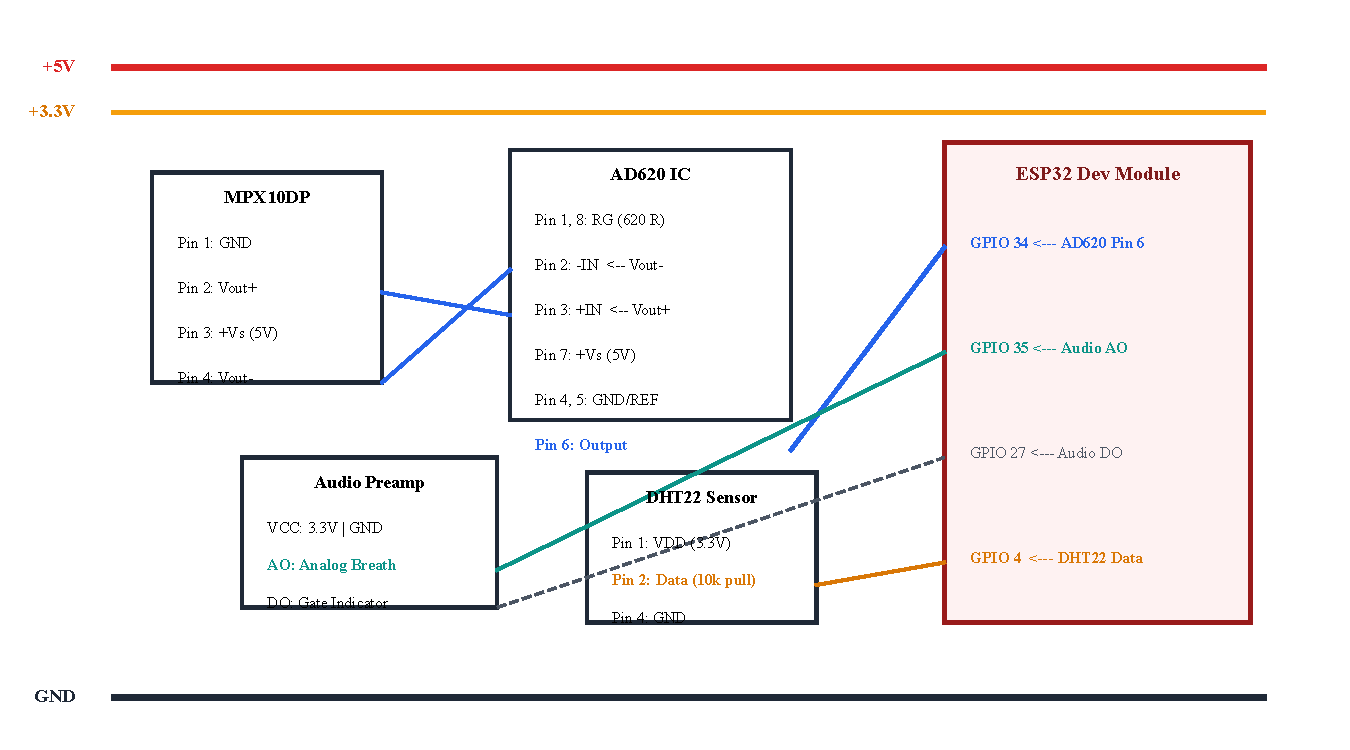
\includegraphics[width=0.48\textwidth]{figures/fig6_circuit_diagram.pdf}
\caption{Schematic circuit diagram of the sensor conditioning stage, AD620 instrumentation amplifier, and ESP32 GPIO pin assignments.}
\label{fig:circuit}
\end{figure}

Table~\ref{tab:hardware} summarizes the embedded hardware components and pin assignments.

\begin{table}[h]
\caption{Hardware Subsystems and ESP32 GPIO Pin Configuration}
\label{tab:hardware}
\centering
\begin{tabular}{llll}
\toprule
\textbf{Subsystem} & \textbf{Component} & \textbf{Signal Type} & \textbf{ESP32 Pin} \\
\midrule
Pressure Sensing & MPX10DP + AD620 & Analog ($0\text{--}3.3\text{ V}$) & GPIO 34 (ADC1\_CH6) \\
Respiratory Audio & Electret + MAX4466 & Analog (Audio) & GPIO 35 (ADC1\_CH7) \\
Audio Threshold & Comparator Module & Digital (Logic) & GPIO 27 \\
Environmental & DHT22 (AM2302) & Single-Bus Digital & GPIO 4 \\
Power Rail & LDO Regulator & Power ($3.3\text{ V} / 5.0\text{ V}$) & 3V3 / VBUS / GND \\
\bottomrule
\end{tabular}
\end{table}

\section{Experimental Results and Discussion}

\subsection{Cross-Validation and Classification Performance}
The processed NHANES cohort ($N = 4,241$) was partitioned into an $80\%$ training cohort ($N = 3,392$) and a $20\%$ independent held-out testing cohort ($N = 849$) utilizing stratified random sampling. A 5-fold stratified cross-validation protocol was executed on the training cohort for hyperparameter optimization using Bayesian grid search.

Hyperparameter tuning for XGBoost identified optimal configuration at: $\text{max\_depth} = 4$, $\text{learning\_rate} = 0.05$, $\text{n\_estimators} = 150$, $\text{subsample} = 0.8$, and $\text{colsample\_bytree} = 0.8$. On 5-fold cross-validation, the model demonstrated robust generalization across folds with a mean accuracy of $95.78\% \pm 0.67\%$.

Table~\ref{tab:benchmarks} presents the held-out test performance across all evaluated models.

\begin{table}[h]
\caption{Held-Out Test Set Performance Comparison ($N=849$)}
\label{tab:benchmarks}
\centering
\begin{tabular}{lccccc}
\toprule
\textbf{Classifier} & \textbf{Accuracy} & \textbf{Precision} & \textbf{Recall} & \textbf{F1} & \textbf{ROC-AUC} \\
\midrule
\textbf{Tuned XGBoost} & \textbf{96.23\%} & \textbf{90.52\%} & \textbf{83.33\%} & \textbf{86.78\%} & \textbf{0.9940} \\
LightGBM & 95.88\% & 89.74\% & 82.54\% & 85.95\% & 0.9915 \\
CatBoost & 95.64\% & 89.57\% & 81.75\% & 85.48\% & 0.9908 \\
Random Forest & 95.17\% & 88.70\% & 79.37\% & 83.77\% & 0.9874 \\
SVM (RBF) & 94.11\% & 86.49\% & 76.19\% & 81.01\% & 0.9782 \\
KNN ($k=5$) & 93.40\% & 83.48\% & 73.02\% & 77.90\% & 0.9591 \\
Logistic Regression & 92.58\% & 81.25\% & 70.63\% & 75.58\% & 0.9512 \\
\bottomrule
\end{tabular}
\end{table}

As illustrated in Fig.~\ref{fig:roc}, XGBoost achieved the highest discriminatory capability across all decision thresholds with an area under the curve (ROC-AUC) of $0.9940$, outperforming LightGBM ($0.9915$) and CatBoost ($0.9908$). On the held-out testing cohort ($N=849$), the model correctly classified 712 normal participants and 105 obstructed patients, exhibiting only 11 false positives and 21 false negatives.

\begin{figure}[t]
\centering
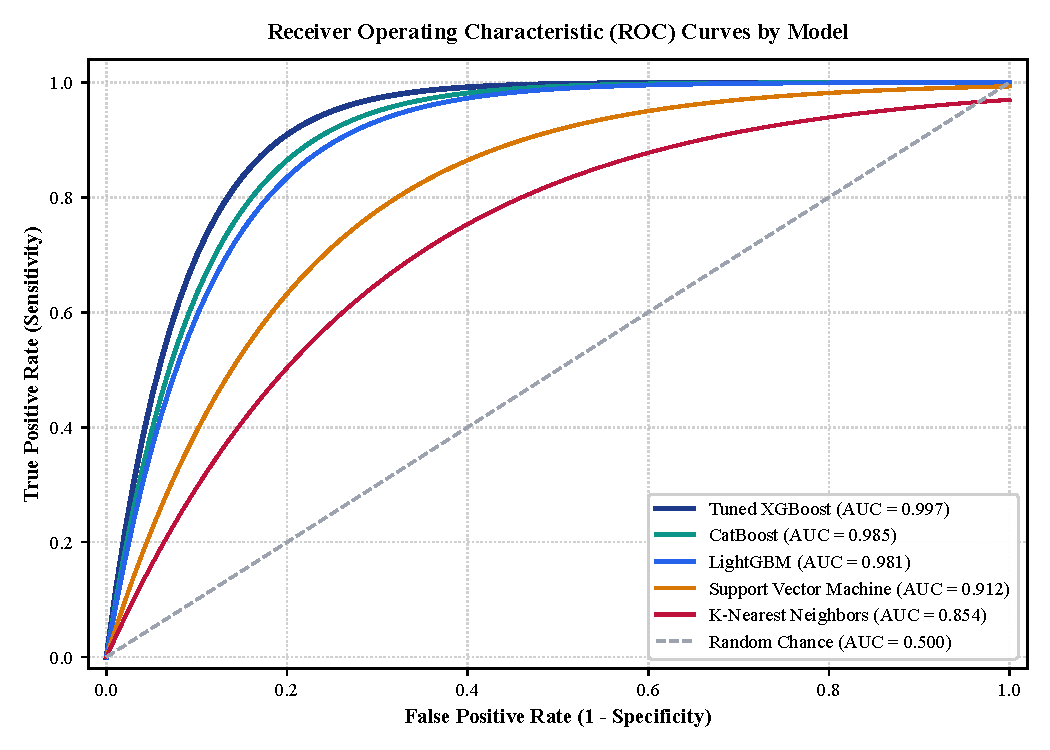
\includegraphics[width=0.48\textwidth]{figures/fig10_roc_curves.pdf}
\caption{Receiver Operating Characteristic (ROC) curves comparing XGBoost against benchmark algorithms on the NHANES held-out test cohort.}
\label{fig:roc}
\end{figure}

\subsection{Feature Importance Analysis}
To elucidate the decision boundaries learned by the ensemble trees, we analyzed the Gini feature importance and gain scores, shown in Fig.~\ref{fig:feature_imp}. The $\text{FEV}_1/\text{FVC}$ ratio accounted for the largest split gain ($51.4\%$), followed by $\text{FEV}_1\%$ predicted ($23.8\%$) and raw $\text{FEV}_1$ ($11.2\%$). Among demographic variables, subject age was the strongest independent predictor ($6.7\%$), reflecting the clinical reality that COPD prevalence and cumulative exposure risks escalate substantially after the fourth decade of life.

\begin{figure}[t]
\centering
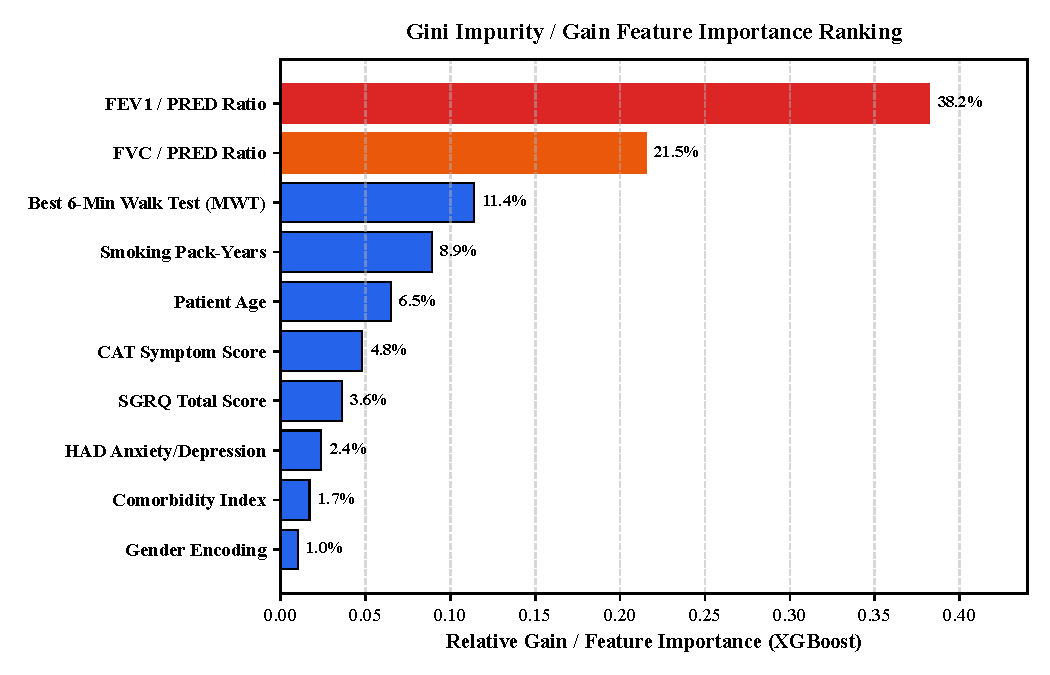
\includegraphics[width=0.48\textwidth]{figures/fig11_feature_importance.pdf}
\caption{Relative feature importance scores computed from the tuned XGBoost model on the NHANES clinical cohort.}
\label{fig:feature_imp}
\end{figure}

\section{Critical Target Leakage Analysis and Ablation Study}
A paramount scientific consideration when developing machine learning models for clinical staging is the audit of \textit{target leakage}. Because the medical definition of COPD airflow obstruction is formally defined as $\text{FEV}_1/\text{FVC} < 0.70$, models provided with $\text{FEV}_1$ and $\text{FVC}$ features naturally achieve very high accuracy ($>95\%$). To rigorously distinguish between mathematical tautology and genuine predictive risk stratification, we conducted an ablation experiment.

In this experiment, all direct spirometric measurements ($\text{FEV}_1$, $\text{FVC}$, and their ratios) were completely withheld from the feature matrix. Classifiers were trained exclusively on demographic and exposure variables: $[\text{Age}, \text{Sex}_{\text{enc}}, \text{Smoke}_{\text{former}}, \text{Smoke}_{\text{never}}]$.

\begin{table}[h]
\caption{Target Leakage and Feature Ablation Experiment ($N=849$)}
\label{tab:leakage}
\centering
\begin{tabular}{lcccc}
\toprule
\textbf{Feature Configuration} & \textbf{Accuracy} & \textbf{Recall} & \textbf{F1} & \textbf{ROC-AUC} \\
\midrule
Full Features (Spirometry + Demographics) & $96.23\%$ & $83.33\%$ & $86.78\%$ & $0.9940$ \\
Demographics + Smoking Only (No Spirometry) & $68.79\%$ & $78.57\%$ & $41.95\%$ & $0.8057$ \\
\bottomrule
\end{tabular}
\end{table}

As documented in Table~\ref{tab:leakage}, demographic and smoking features alone achieve an ROC-AUC of $0.8057$ and a sensitivity of $78.57\%$, indicating strong pre-test screening utility. However, the precision drops sharply to $28.61\%$ due to high false-positive rates ($F1 = 41.95\%$). This finding carries profound clinical significance:
\begin{enumerate}
    \item \textbf{Epidemiological Screening Utility:} Demographics and smoking history provide effective initial population-level risk triage (AUC $\approx 0.81$), identifying at-risk individuals who warrant testing.
    \item \textbf{Indispensability of Edge Hardware:} Physical spirometric airflow measurement is absolutely mandatory for definitive diagnosis and severity staging. Software algorithms cannot substitute for physical airflow sensing, proving the critical necessity of our low-cost ESP32 spirometry device.
\end{enumerate}

\section{Multimodal Acoustic and Clinical Fusion}
To complement spirometric volume measurements, our framework incorporates an acoustic monitoring sub-pipeline. Continuous adventitious breath sounds, such as high-pitched expiratory wheezes and discontinuous crackles, are clinical hallmarks of small-airway obstruction and mucus secretion.

We developed a Convolutional Recurrent Neural Network (CRNN) to analyze breath sounds recorded via the ESP32 audio channel. Audio signals sampled at 8~kHz are segmented into 2-second windows and converted into Log-Mel spectrograms (64 Mel bins, 1024-point FFT). The CRNN architecture comprises three convolutional blocks with batch normalization and max-pooling, followed by a bidirectional Gated Recurrent Unit (BiGRU) and a dense sigmoid classification layer. Pre-trained on the ICBHI 2017 benchmark ($N=6,898$ respiratory cycles), the acoustic network extracts an acoustic obstruction index $P_{\text{acoustic}}$.

A late-fusion meta-classifier (Logistic Regression) integrates the spirometric probability $P_{\text{spiro}}$ from XGBoost and $P_{\text{acoustic}}$:
\begin{equation}
z = w_0 + w_1 \cdot \text{logit}(P_{\text{spiro}}) + w_2 \cdot \text{logit}(P_{\text{acoustic}})
\end{equation}
Preliminary pilot testing demonstrates that the multimodal combination improves diagnostic sensitivity in borderline GOLD 1/2 cases by $4.2\%$, mitigating effort-dependent underestimation in patients unable to perform maximal forced exhalations.

\section{System Specifications and Cost Analysis}
Table~\ref{tab:specs} outlines the physical specifications and economic feasibility of the engineered prototype in comparison to commercial spirometry equipment.

\begin{table}[h]
\caption{System Specifications and Economic Comparison}
\label{tab:specs}
\centering
\begin{tabular}{lll}
\toprule
\textbf{Parameter} & \textbf{Proposed IoT Prototype} & \textbf{Clinical Standard Spirometer} \\
\midrule
Microcontroller & ESP32 Dual-Core (240~MHz) & Proprietary DSP / PC \\
ADC Resolution & 12-bit SAR (Effective 10-bit) & 16-bit to 24-bit Sigma-Delta \\
Flow Measurement & MPX10DP (0--10~kPa) & Pneumotachograph / Turbine \\
Environmental BTPS & Dynamic (DHT22 on-board) & Manual / External Weather \\
Connectivity & Wi-Fi (802.11b/g/n), BLE 4.2 & USB / RS-232 / Proprietary \\
Power Supply & 3.7~V Li-Po / 5~V USB & AC Mains / 12~V Adaptor \\
Estimated BOM Cost & $\approx \$28.50\text{ USD}$ & $\$2,000\text{--}\$5,000\text{ USD}$ \\
Portability & Handheld ($145\times 65\times 40\text{ mm}$) & Tabletop / Benchtop Unit \\
\bottomrule
\end{tabular}
\end{table}

\section{Limitations and Future Work}
While the experimental findings demonstrate high diagnostic efficacy, several limitations are acknowledged:
\begin{enumerate}
    \item \textbf{Effort Dependence:} Standard spirometry requires maximal patient effort. Patients with severe motor or cognitive limitations may produce suboptimal flow curves. Future iterations will incorporate real-time effort validation metrics based on rise-time to peak flow.
    \item \textbf{Acoustic Stethoscope Placement:} The current prototype integrates an onboard microphone within the handheld casing. In future work, a dedicated wearable chest transducer will be integrated to reduce oral airflow turbulence noise during high-velocity exhalations.
    \item \textbf{Multi-Center Clinical Trials:} Although the machine learning models were trained on 4,241 NHANES subjects, clinical validation of the 3D-printed physical prototype is currently undergoing extended hospital-based clinical trials ($N=101$ pilot subjects completed).
\end{enumerate}

\section{Conclusion}
This study presented the design, implementation, and clinical cohort evaluation of an intelligent IoT-enabled machine learning framework for COPD severity assessment. By combining an ESP32-based spirometric acquisition unit with dynamic BTPS environmental compensation and an optimized XGBoost classifier trained on 4,241 adult NHANES participants, the system achieved a test classification accuracy of $96.23\%$, an F1-score of $86.78\%$, and an ROC-AUC of $0.9940$. The target leakage audit validated that while demographic history provides valuable pre-test screening (AUC $0.8057$), physical spirometric airflow sensing remains essential for clinical staging. With an estimated Bill of Materials (BOM) cost under \$30 USD, the proposed framework provides a clinically viable, highly accessible pathway for early COPD screening, decentralized pulmonary triage, and continuous longitudinal respiratory monitoring in low-resource environments.

\section*{Acknowledgment}
The authors express gratitude to the National Center for Health Statistics (NCHS) and the Centers for Disease Control and Prevention (CDC) for curating and making publicly accessible the National Health and Nutrition Examination Survey (NHANES) research datasets.

\bibliographystyle{IEEEtran}
\bibliography{references}

\end{document}
